%! Author = Jakub Hvolka
%! Date = 09/04/2021

% Preamble
\documentclass[a4paper,slovak,12pt]{article}


% Language packages
\usepackage[T1]{fontenc}
\usepackage[utf8]{inputenc}
\usepackage[slovak]{babel}
\usepackage{lmodern}

\usepackage[a4paper,left=1.8cm,right=1.8cm,top=2cm,bottom=2.5cm]{geometry}

% Packages
\usepackage{amsmath}
\usepackage{listings}
\usepackage{xcolor}
\usepackage{multirow}
\usepackage{array}
\usepackage{microtype}
\usepackage{makecell}
\usepackage{pdfpages}
\usepackage{fancyhdr}
\usepackage{indentfirst}
\usepackage{hyperref}
\usepackage{graphicx}
\usepackage{siunitx}
\usepackage{placeins}
\usepackage{caption}
\usepackage{booktabs}
\usepackage{ulem}
\usepackage{color}
\usepackage[bottom]{footmisc}
\usepackage{tikz}
\usepackage{tikz-qtree}

\pdfminorversion=7

\definecolor{mGreen}{rgb}{0,0.4,0}
\definecolor{mGray}{rgb}{0.5,0.5,0.5}
\definecolor{mPurple}{rgb}{0.58,0.0,0.5}
\definecolor{mOrange}{rgb}{.5,0.25,0}

\lstdefinestyle{CPPStyle}{
    basicstyle=\ttfamily,
    commentstyle=\color{mGreen},
    keywordstyle=\color{mPurple},
    numberstyle=\tiny\color{mGray},
    stringstyle=\color{mPurple},
    basicstyle=\footnotesize,
    breakatwhitespace=false,
    breaklines=true,
    captionpos=b,
    keepspaces=true,
    numbers=left,
    numbersep=5pt,
    showspaces=false,
    showstringspaces=false,
    showtabs=false,
    tabsize=4,
    language=C++
}


\newcolumntype{?}{!{\vrule width 1pt}}

% \cline fix found here: https://tex.stackexchange.com/questions/111999/slovak-and-czech-babel-gives-problems-with-cmidrule-and-cline
\makeatletter
\begingroup
\toks0=\expandafter{\@cline{#1}-{#2}\@nil}
\@ifpackageloaded{booktabs}{%
    \toks2=\expandafter{\@@@cmidrule[{#1}-{#2}]{#3}{#4}}%
}{}
\catcode`-=\active
\edef\x{\gdef\unexpanded{\@cline#1-#2\@nil}{\the\toks0}}\x
\@ifpackageloaded{booktabs}{%
    \edef\x{\gdef\unexpanded{\@@@cmidrule[#1-#2]#3#4}{\the\toks2}}\x
}{}
\endgroup
\makeatother

\renewcommand{\headrulewidth}{.4mm} % header line width

\pagestyle{fancy}
\fancyhf{}
\fancyhfoffset[L]{1cm} % left extra length
\fancyhfoffset[R]{1cm} % right extra length
\lhead{\color{darkgray}Jakub Hvolka: 110801, ak. rok 2020/2021}
\lfoot{\color{darkgray}Zadanie č. 2 – Vyhľadávanie v dynamických množinách }
\rfoot{\thepage}


\setlength{\parskip}{1em}


% Document
\begin{document}

    \begin{titlepage}
        \begin{center}
            \Large
            Slovenská technická univerzita v Bratislave\\

            Fakulta informatiky a informačných technológií

            \vspace*{\fill}

            \huge
            Dátové štruktúry a algoritmy\\
            \large
            Zadanie č. 2 – Vyhľadávanie v dynamických množinách


            \vspace*{\fill}

            Jakub Hvolka\\
            ID:110801\\
            ak.rok 2020/2021
            \vspace*{2cm}

        \end{center}
    \end{titlepage}

    \tableofcontents

    \newpage


    \section{Opis algoritmu}\label{sec:opis-algoritmu}

    \subsection{Prevzaté implementácie}\label{subsec:prevzate-implementacie}
    Algoritmy som prevzal zo stránky GitHub.
    Konkrétne \href{https://github.com/Travelinglight/AVLTree/blob/master/AVLTree.h}{AVL strom}\footnote{\url{https://github.com/Travelinglight/AVLTree/blob/master/AVLTree.h}}
    a \href{https://gist.github.com/Ashwin-op/70581aba99c793d64a2e428e72786ab0}{hash tabuľku s reťazením}\footnote{\url{https://gist.github.com/Ashwin-op/70581aba99c793d64a2e428e72786ab0}}.

    Zdrojový kód hash tabuľky som musel upraviť:
    \begin{itemize}
        \item celý kód som vložil do namepsace HashSC keďže došlo ku kolízii s menami z iných dátových štruktúr,
        \item vymenil som typ hodnôt z \textbf{int} na \textbf{size\_t} aby bol pri testovaní všade rovnaký,
        \item  a odstránil som funkciu main.
    \end{itemize}

    \subsection{Vlastné implementácie}\label{subsec:vlastne-implementacie}

    V mojich implementáciách som vytvoril len funkcie potrebné na vloženie a vyhľadanie dát v štruktúrach a na
    uvoľnenie pamäti.

    \subsubsection{Binárny vyhľadávací strom}\label{subsubsec:cerveno-cierny-strom}

    Moja implementácia BVS je červeno-čierny strom.

    \paragraph{Vkladanie:}
    Funkcia vytvorí nový prvok, ktorý následne vloží do stromu ako list.
    Nový prvok je označený ako červený.

    Keďže nový prvok je červený, môže nastať porušenie vlastností červeno-čierneho stromu,
    konkrétne faktu, že dva červené prvky nesmú byť za sebou.
    Funkcia opakuje nasledujúce kroky, pokiaľ neplatia všetky vlastnosti červeno-čierneho stromu.
    Jednotlivé situácie sú rozdelené symetricky podľa toho, či je rodiť pravé alebo ľavé dieťa.
    Uvediem kroky pre prípad, keď je rodič ľavé dieťa:
    \begin{enumerate}
        \item Ak je aktuálny prvok koreň stromu, nastav ho na čierny.
        Všetky vlastnosti platia a cyklus sa môže ukončiť.
        \item Ak je rodič a rodičov súrodenec červený, nastav ich farbu na čierny a prarodiča na červeného.
        Pokračuj od začiatku s prarodičom.
        \item Ak aktuálny prvok je pravé dieťa, otoč ho doľava.
        Keďže aktuálny prvok aj jeho rodič sú červený (ak by nebol červený, nenastalo by porušenie vlastností), rotácia
        nezmení aktuálny stav porušených vlastností.
        Pokračuj nasledujúcim krokom.
        \item Keďže aktuálny prvok je červene ľavé dieťa, jeho rodič je tiež červený.
        To znamená, že prarodič je čierny.
        Nastav farbu rodiča na čiernu a prarodiča na červenú.
        Otoč prarodiča doprava.
        Všetky vlastnosti platia a cyklus sa môže ukončiť.
    \end{enumerate}
    Naviac, ak je aktuálny prvok koreň stromu, nastav ho na čierny.
    Všetky vlastnosti platia a cyklus sa môže ukončiť.

    \subsubsection{Hash tabuľka}\label{subsubsec:hash-tabulka-s-retazenim}

    Implementoval som tabuľku s otvoreným reťazením.
    Na hľadanie pozície som použil lineárne skúšanie, s Robinhood hashing.

    Veľkosť tabuľky je vždy rovná $2^k$ aby som miesto funkcie modulo mohol použiť bitovú masku.

    \paragraph{Hash funkcia:}
    Použil som polynóm štvrtého stupňa modulo $2^{31}-1$ aby som zabezpečil, že moja hash funkcia je zo
    silno univerzálnej\textsubscript{5} hash rodiny funkcií
    \footnote{Wegman, Mark N.; Carter, J. Lawrence (1981). "New hash functions and their
    use in authentication and set equality"  Journal of Computer and System Sciences. 22 (3): 265–279. doi:10.1016/0022-0000(81)90033-7},
    potrebnej na zabezpečenie konštantného času operácií pri použití lineárneho skúšania\footnote{Pagh, Anna; Pagh, Rasmus; Ružić, Milan (2009),
        "Linear probing with constant independence",
        SIAM Journal on Computing, 39 (3): 1107–1120, arXiv:cs/0612055, doi:10.1137/070702278, MR 2538852}.\hfill

    \paragraph{Vkladanie:}
    Na žačiatku sa skontroluje, či faktor naplnenia nepresahuje hodnotu 90\%.
    Ak áno, vytvorí sa nová tabuľka a prvky z pôvodnej tabuľky sa do nej vložia.

    Následne sa vypočíta hash pre vkladaný kľúč a aplikovaním bitovej masky ideálna pozícia pre vloženie.
    Ak miesto na danej pozícii nie je voľné, algoritmus skúša postupne nasledujúce miesta v pamäti, až kým voľné miesto nenájde.

    Taktiež som implementoval Robinhood hashing, ktoré spočíva v minimalizácii vzdialenosti prvkov od ich ideálneho miesta.
    Vzdialenosťou od ideálneho miesta nazvem vzdialenosť adresy od adresy získanej hashovaním kľúča a aplikovaním bitovej masky.
    Pri každej kolízii, algoritmus porovná vzdialenosti od ideálneho miesta vkladaného prvku a prvku s ktorým nastala kolízia.
    Na aktuálnej pozícii nechá prvok z väčšou vzdialenosťou od ideálneho miesta, a ďalej posúva zvyšný.

    \paragraph{Vyhľadávanie:}
    Podľa kľúča sa nájde ideálne miesto na ktorom sa môže prvok nachádzať.
    Následne sa postupne porovnávajú kľúče uložené na adrese od ideálneho miesta, pokiaľ sa nenájde zhodný kľúč, alebo prázdne miesto.
    Ak sa nájde zhodný kľúč, funkcia vráti hodnotu.

    Funkcia sa vždy ukončí, keďže v tabuľke je vždy aspoň 10\% prázdnych miest.


    \section{Spôsob testovania}\label{sec:sposob-testovania}

    Na testovanie som vytvoril jednu funkciu (šablónu, podľa typu skúšanej triedy).
    Táto funkcia je rozdelená na dve časti.

    Prvá časť (v kóde označovaná \textit{assignment\_compliant}) meria časy potrebné na vykonanie všetkých operácií za sebou, podľa
    prílohy B v sekcii~\ref{sec:priloha-b-upresnenie-znenia-zadania-c-2}.

    Druhá časť meria časy jednotlivých operácii v skupinách.
    Pri testovaní som nastavil veľkosť skupiny na 100.

    Pre jednotlivé testy sa po spustení programu vytvoria dve sady hodnôt na testovanie.
    Jedna obsahuje zoradenú postupnosť čísel od 1, a druhá obsahuje náhodné čísla.
    Postupnosť náhodných čísel je vytvorená z postupnosti unikátnych čísel, ktorá je následne zamiešaná.

    Jednotlivé testované funkcie som obalil do labmda funkcií, líšiacich sa len typom štruktúry, aby som umožnil použitie
    tej istej funkcie (šablóny) pre rôzne dátové štrkutúry s rôznymi názvami daných funkcií.

    Na meranie časov vykonávania meraných funkcií som implementoval triedu Timer.
    Táto trieda sa stará o meranie trvaní, ich ukladanie a výpis do csv (čiarkou oddelené hodnoty) súboru, ako aj sumárny výpis do konzoly.
    Výsledné dáta sú spracované a zobrazené v nasledujúcej sekcii~\ref{sec:dosiahnute-vysledky}.
    Na spracovanie dát som použil program Excel.
    Spracovanie zahŕňa spriemerovanie časov behov jednotlivých meraní a výpočet priemerného času pre jednu operáciu.

    Pri testovaní som použil kompilátor MSVC s \textbackslash{}Od možnosťou, aby som zabránil optimalizácii, ktorá by odstránila niektoré merané funkcie.

    \section{Dosiahnuté výsledky}\label{sec:dosiahnute-vysledky}

    Oba vyhľadávacie stromy majú logaritmickú zložitosť pri vkladaní aj vyhľadávaní.
    Moja implementácia je rýchlejšia pri oboch operáciách

    Hash tabuľky majú obe očakávanú konštantnú časovú zložitosť pri oboch operáciách.
    Obe implementácie sú podobne rýchle.
    Prevzatá implementácia je pri mojom testovaní o málo rýchlejšia pri vyhľadávaní a pomalšia pri vkladaní, oproti mojej implementácii.

    Obe hash tabuľky potrebujú veľa času na zväčšenie tabuľky.
    Na grafoch hash tabuliek je to vidno ako veľké časové hodnoty, ktoré exponenciálne rastú s exponenciálne veľkými medzerami medzi sebou.
    Keďže obe implementácie používajú geometrický nárast, obe implementácie majú amortizovanú konštantnú časovú zložitosť aj
    pri rozširovaní tabuľky.

    \FloatBarrier
    \begin{table}[!htbp]
        \centering
        \fontsize{9.5}{13}
        \selectfont
        \caption{Červeno - čierny strom}
        \label{tab:cerveno-cierny-strom}
        \setlength{\tabcolsep}{2.7pt}
        \begin{tabular} {c|ccc|ccc||cc|cc}
            \toprule
            \multirow{3}{*}{\makecell{počet \\operácií}} & \multicolumn{6}{c||}{Insert v nano sekundách} & \multicolumn{4}{c}{Search v nanosekundách} \\
            & \multicolumn{3}{c|}{Usporiadaný vstup} & \multicolumn{3}{c||}{Náhodný vstup} & \multicolumn{2}{c|}{Usporiadaný vstup}
            & \multicolumn{2}{c}{Náhodný vstup}
            \\
            & Vytvorenie   & 1 prvok & 25\% prvkov   & Vytvorenie   & 1 prvok & 25\% prvkov   & 1 prvok & 5\% prvok
            & 1 prvok
            & 5\% prvok
            \\ \midrule
            1000  &  158540 & 158,54 & 44480 & 179180 & 179,18 & 44740 & 44,5 & 2360 & 49,8 & 2500      \\
            25000 &  5066760 & 202,6704 & 1284080 & 6718780 & 268,7512 & 1951980 & 69,4096 & 85900 & 65,7024 & 84000    \\
            100000 & 20478520 & 204,7852 & 5510300 & 31509700 & 315,097 & 9203440 & 73,942 & 374380 & 64,7426 & 319620  \\ \bottomrule
        \end{tabular}
    \end{table}

    \begin{table}[!htbp]
        \centering
        \fontsize{9.5}{13}
        \selectfont
        \caption{AVL strom}
        \label{tab:avl-strom}
        \setlength{\tabcolsep}{2.7pt}
        \begin{tabular} {c|ccc|ccc||cc|cc}
            \toprule
            \multirow{3}{*}{\makecell{počet \\operácií}} & \multicolumn{6}{c||}{Insert v nano sekundách} & \multicolumn{4}{c}{Search v nanosekundách} \\
            & \multicolumn{3}{c|}{Usporiadaný vstup} & \multicolumn{3}{c||}{Náhodný vstup} & \multicolumn{2}{c|}{Usporiadaný vstup}
            & \multicolumn{2}{c}{Náhodný vstup}
            \\
            & Vytvorenie   & 1 prvok
            & 25\% prvkov   & Vytvorenie   & 1 prvok & 25\% prvkov   & 1 prvok & 5\% prvok
            & 1 prvok
            & 5\% prvok
            \\ \midrule
            1000  &  499940 & 499,94 & 131820 & 587840 & 587,84 & 178180 & 110,98 & 7700 & 156,26 & 7920    \\
            25000 &  14712340 & 588,4936 & 3920340 & 20246200 & 809,848 & 5715780 & 141,1464 & 292500 & 271,8624 & 356140  \\
            100000 & 61321760 & 613,2176 & 16368380 & 91178360 & 911,7836 & 25627980 & 149,7174 & 1318460 & 323,8394 & 1637800  \\\bottomrule
        \end{tabular}
    \end{table}
    \begin{table}[!htbp]
        \centering
        \fontsize{9.5}{13}
        \selectfont
        \caption{Hashovacia tabuľka otvorené adresovanie}
        \label{tab:hashovacia-tabulka-otvorene-adresovanie}
        \setlength{\tabcolsep}{2.7pt}
        \begin{tabular} {c|ccc|ccc||cc|cc}
            \toprule
            \multirow{3}{*}{\makecell{počet \\operácií}} & \multicolumn{6}{c||}{Insert v nano sekundách} & \multicolumn{4}{c}{Search v nanosekundách} \\
            & \multicolumn{3}{c|}{Usporiadaný vstup} & \multicolumn{3}{c||}{Náhodný vstup} & \multicolumn{2}{c|}{Usporiadaný vstup}
            & \multicolumn{2}{c}{Náhodný vstup}
            \\
            & Vytvorenie   & 1 prvok
            & 25\% prvkov    & Vytvorenie   & 1 prvok & 25\% prvkov    & 1 prvok  & 5\% prvok
            & 1 prvok
            & 5\% prvok
            \\ \midrule
            1000  &  189700 & 189,7 & 28420 & 274800 & 274,8 & 33020 & 99,52 & 5100 & 99,66 & 4920 \\
            25000 &  4855260 & 194,2104 & 2453420 & 5346160 & 213,8464 & 2579520 & 117,5616 & 155800 & 119,9 & 145400   \\
            100000 & 20401300 & 204,013 & 10513760 & 22935280 & 229,3528 & 11803240 & 120,1428 & 584260 & 120,7554 & 614360 \\ \bottomrule
        \end{tabular}
    \end{table}
    \begin{table}[!htbp]
        \centering
        \fontsize{9.5}{13}
        \selectfont
        \caption{Hashovacia tabuľka reťazenie}
        \label{tab:hashovacia-tabulka-retazenie}
        \setlength{\tabcolsep}{2.7pt}
        \begin{tabular} {c|ccc|ccc||cc|cc}
            \toprule
            \multirow{3}{*}{\makecell{počet \\operácií}} & \multicolumn{6}{c||}{Insert v nano sekundách} & \multicolumn{4}{c}{Search v nanosekundách} \\
            & \multicolumn{3}{c|}{Usporiadaný vstup} & \multicolumn{3}{c||}{Náhodný vstup} & \multicolumn{2}{c|}{Usporiadaný vstup}
            & \multicolumn{2}{c}{Náhodný vstup}
            \\
            & Vytvorenie   & 1 prvok
            & 25\% prvkov    & Vytvorenie   & 1 prvok & 25\% prvkov    & 1 prvok  & 5\% prvok
            & 1 prvok
            & 5\% prvok
            \\ \midrule
            1000  &      223280 & 223,28 & 88460 & 246440 & 246,44 & 91320 & 70,38 & 3600 & 105,66 & 5140                    \\
            25000 &     6854120 & 232,69 & 1306560 & 6186660 & 246,42 & 1191400 & 71,51 & 101140 & 124,11 & 204140          \\
            100000 &  23268520 & 274,16 & 4776280 & 24642300 & 247,47 & 4943840 & 77,08 & 475440 & 88,23 & 501760   \\ \bottomrule
        \end{tabular}
    \end{table}

    \FloatBarrier

    Obe implementácie vyhľadávacích stromov majú logaritmickú časovú zložitosť pri vkladaní.

    Na grafoch sú červenou vyznačené časy pri použití náhodne generovaných čísel, a modrou pre postupnosť čísel.

    \FloatBarrier

    \begin{figure}[!htbp]
        \centering
        \label{fig:figure1}
        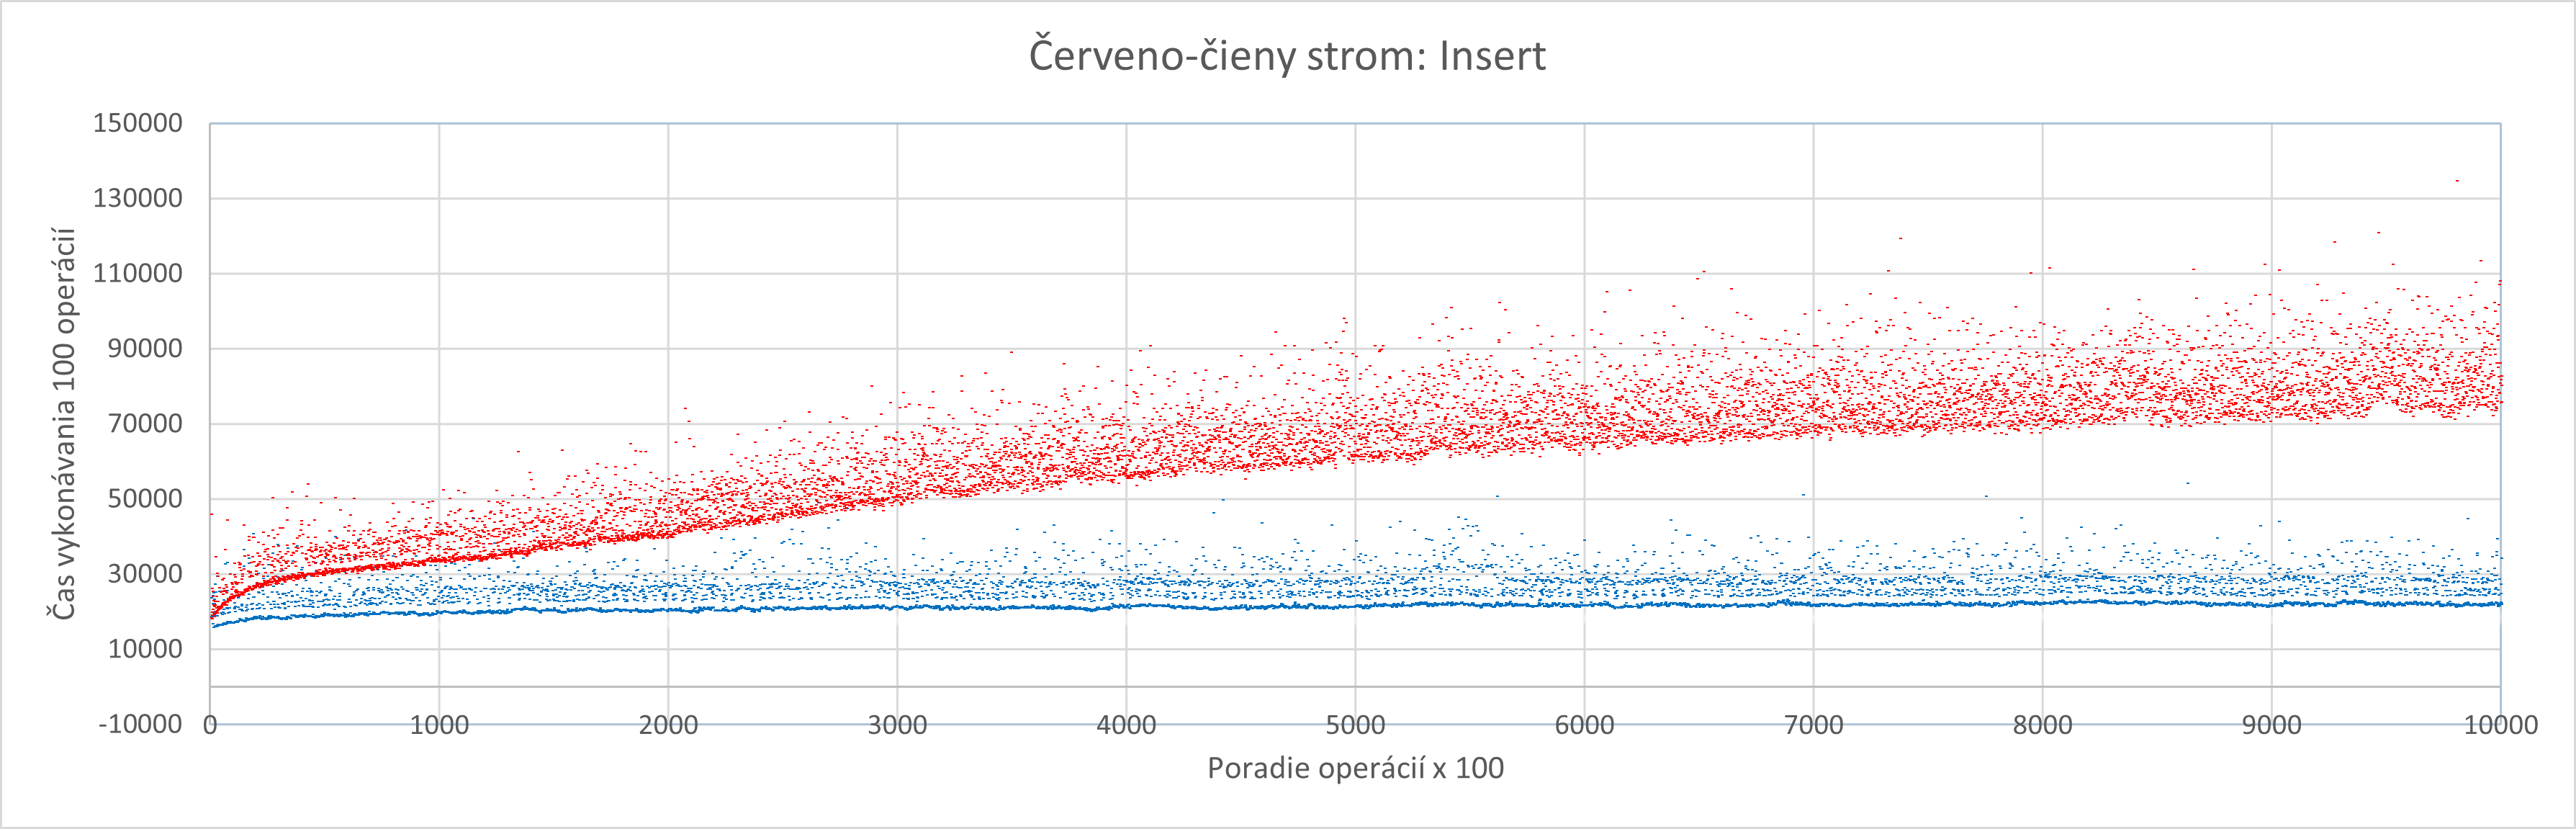
\includegraphics[width=\textwidth]{RB_Insert}
    \end{figure}
    \begin{figure}[!htbp]
        \centering
        \label{fig:figure2}
        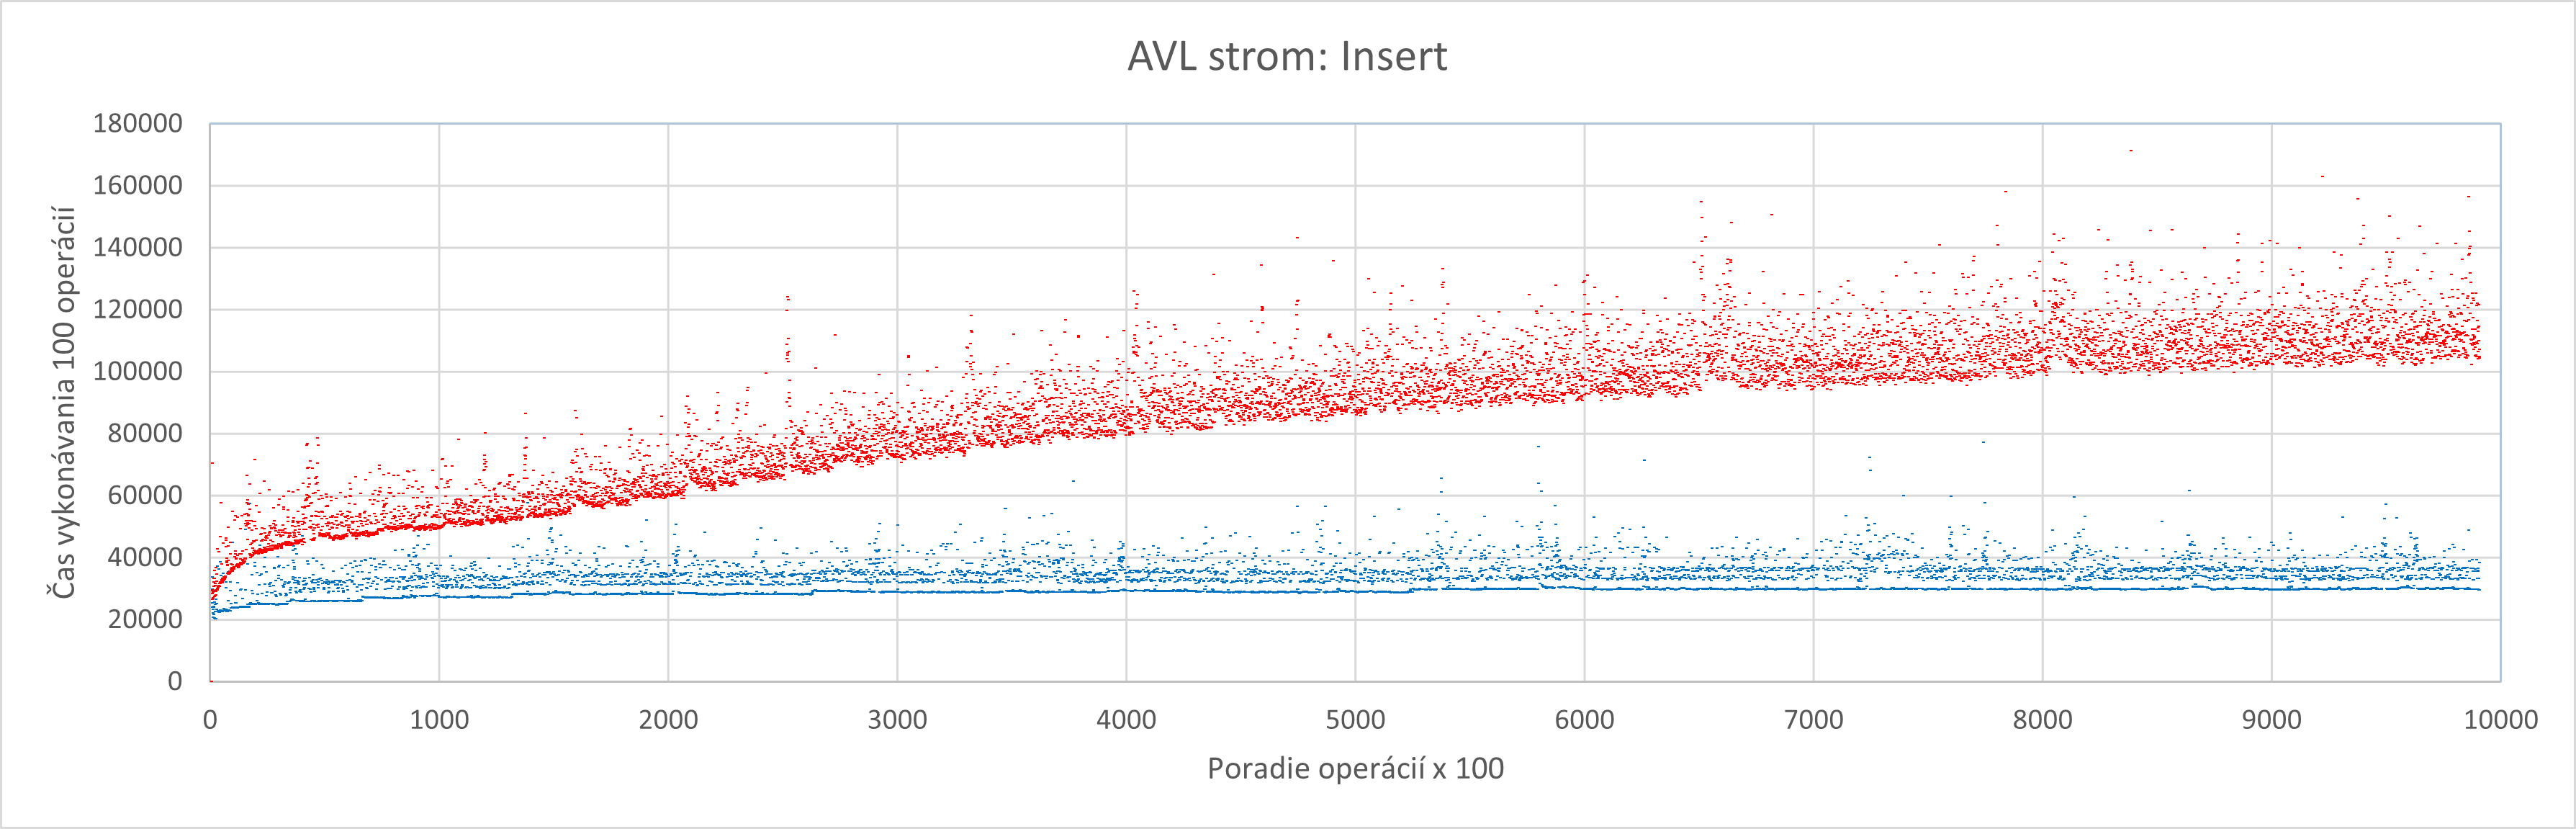
\includegraphics[width=\textwidth]{AVL_Insert}
    \end{figure}
    \begin{figure}[!htbp]
        \centering
        \label{fig:figure3}
        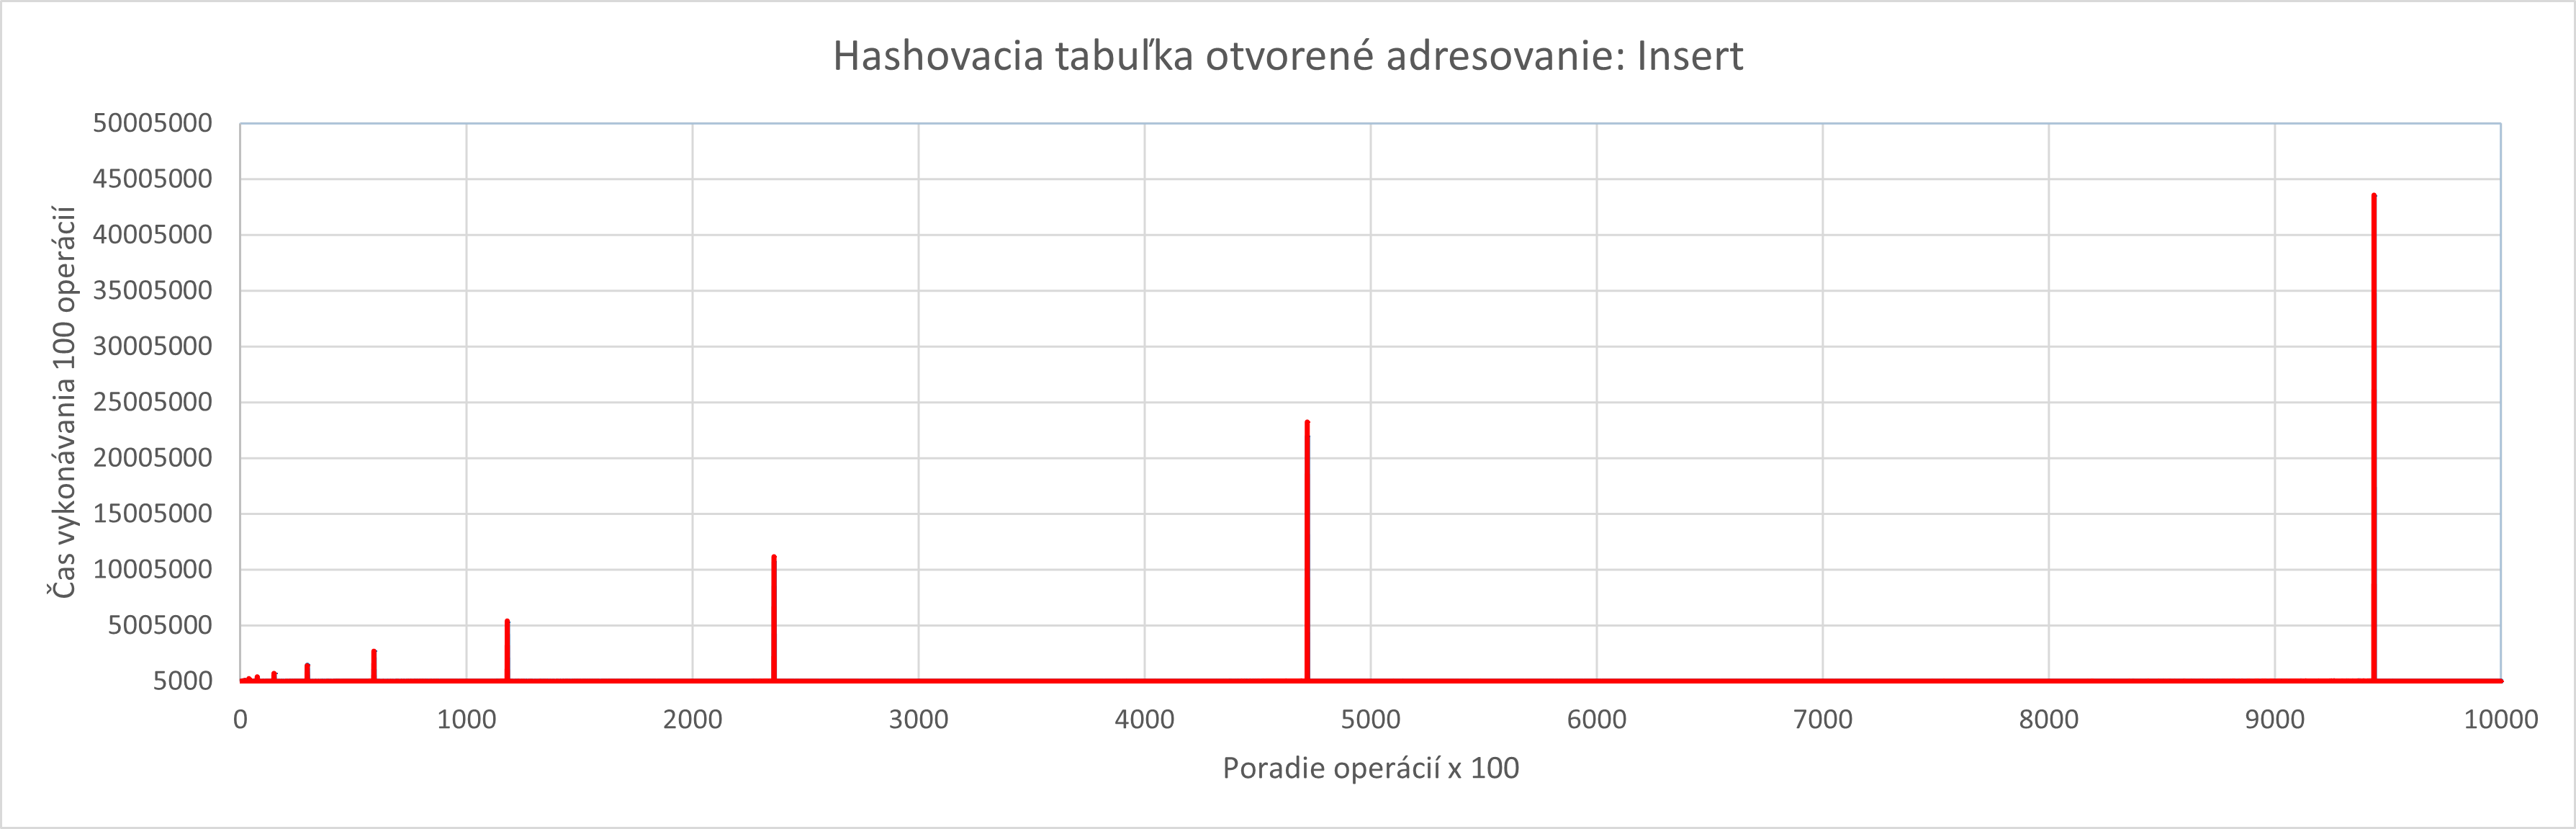
\includegraphics[width=\textwidth]{HashRobin_Insert}
    \end{figure}
    \begin{figure}[!htbp]
        \centering
        \label{fig:figure4}
        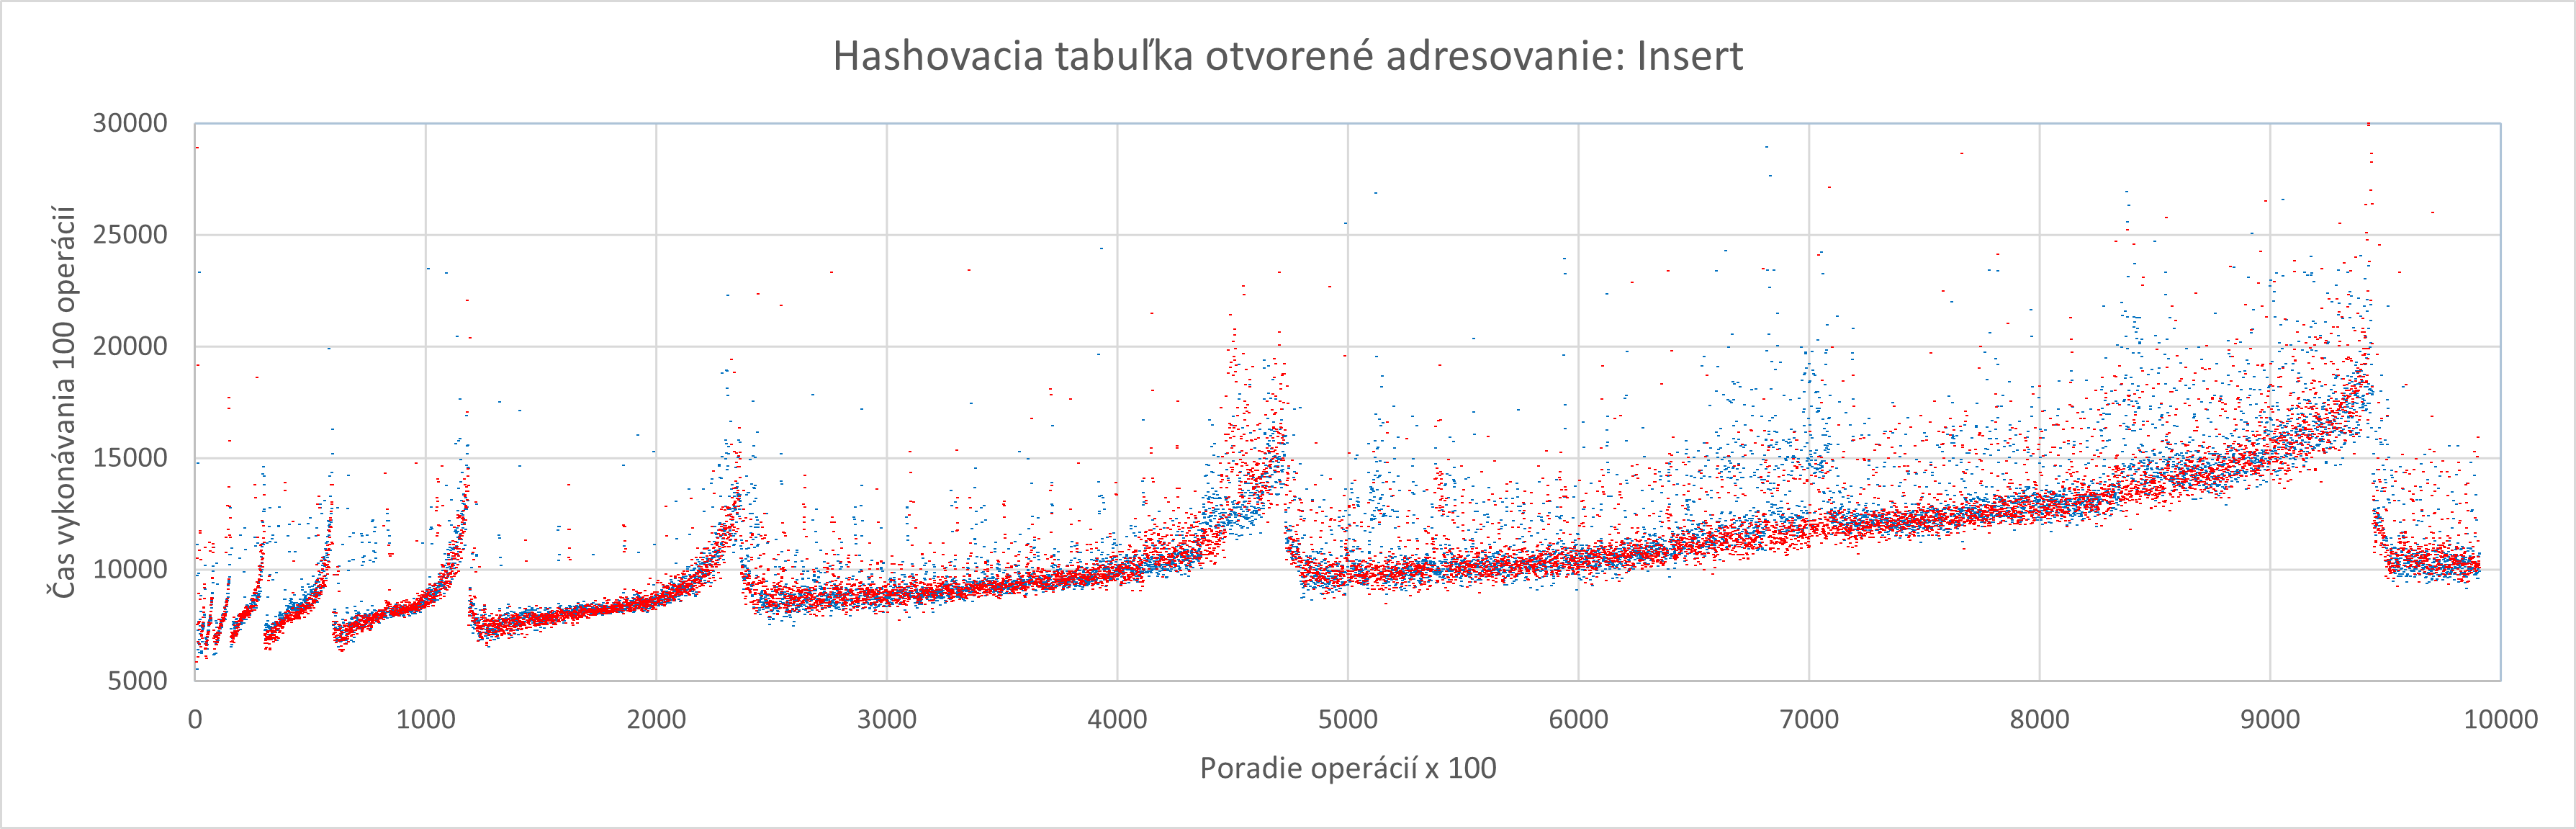
\includegraphics[width=\textwidth]{HashRobin_Insert_zoomed}
    \end{figure}
    \begin{figure}[!htbp]
        \centering
        \label{fig:figure5}
        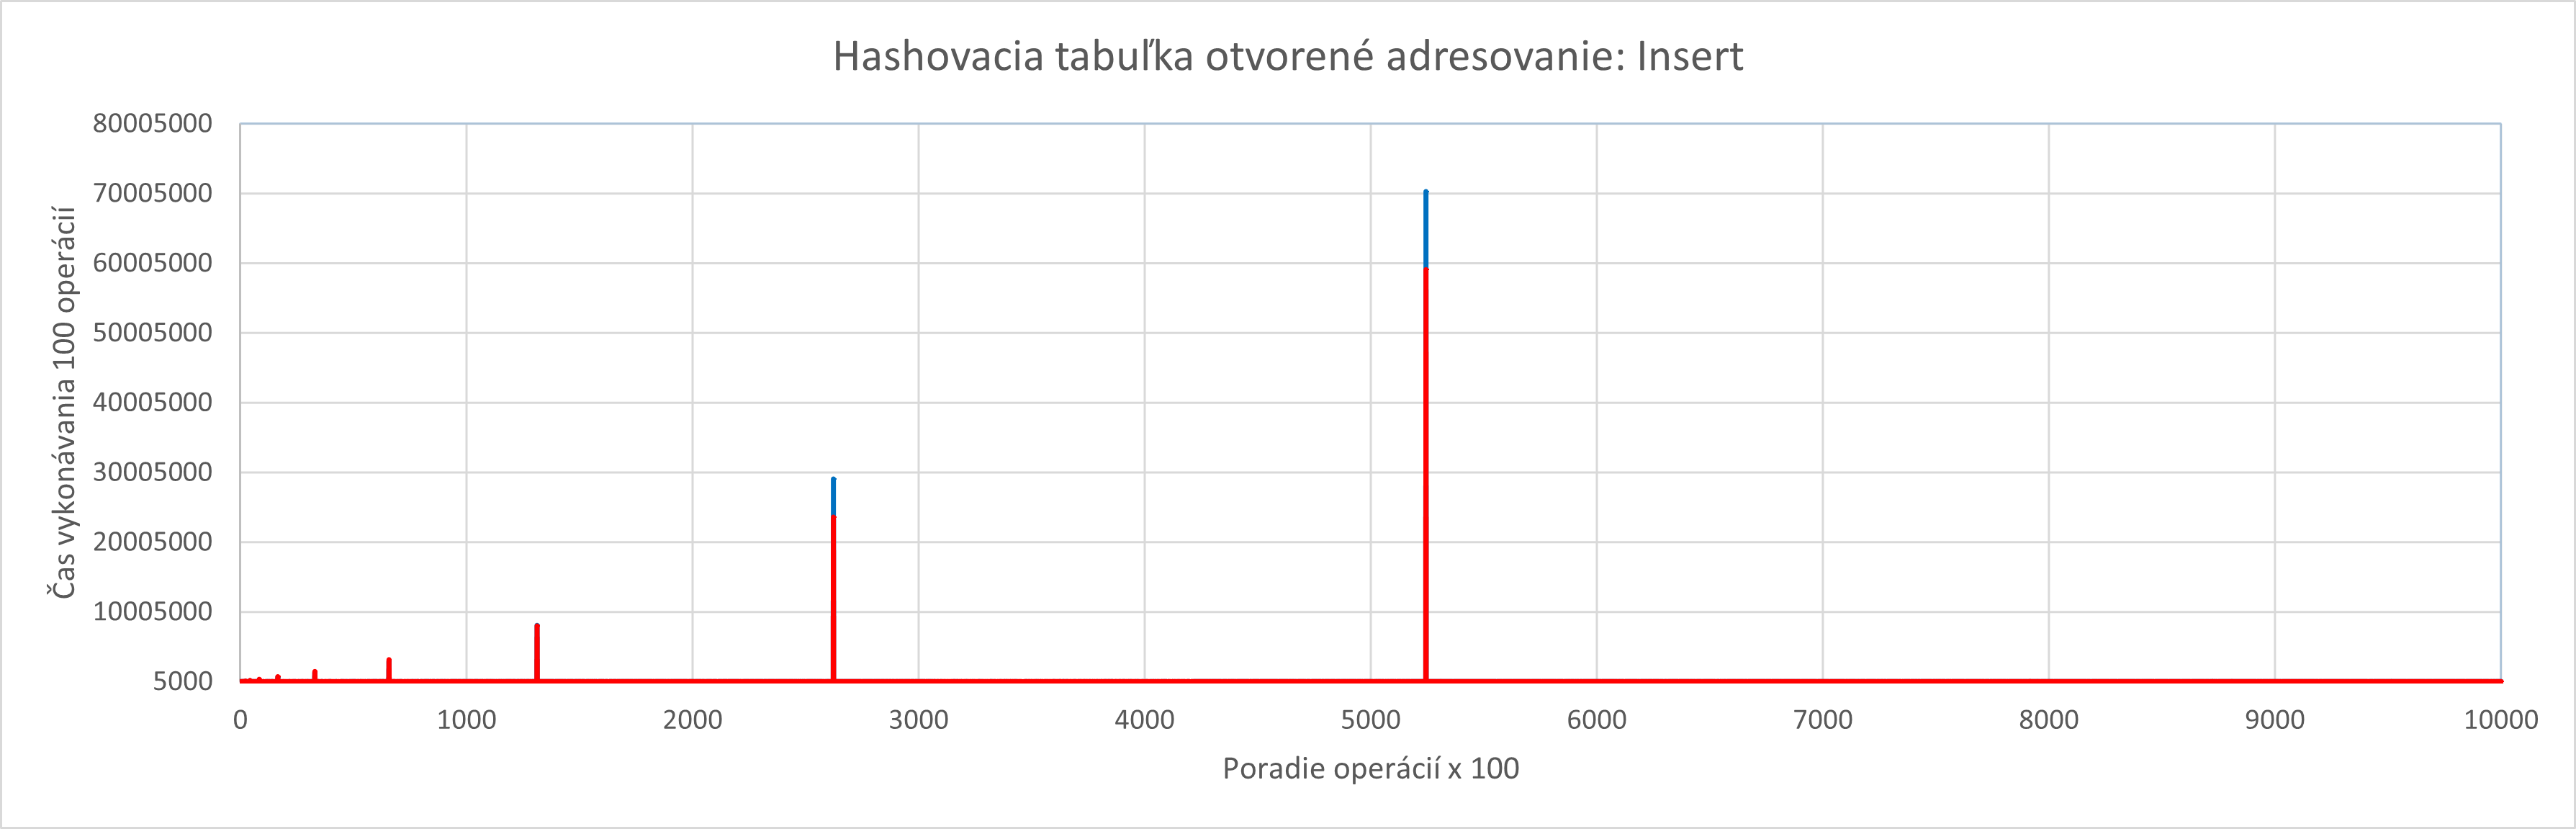
\includegraphics[width=\textwidth]{HashSC_Insert}
    \end{figure}
    \begin{figure}[!htbp]
        \centering
        \label{fig:figure6}
        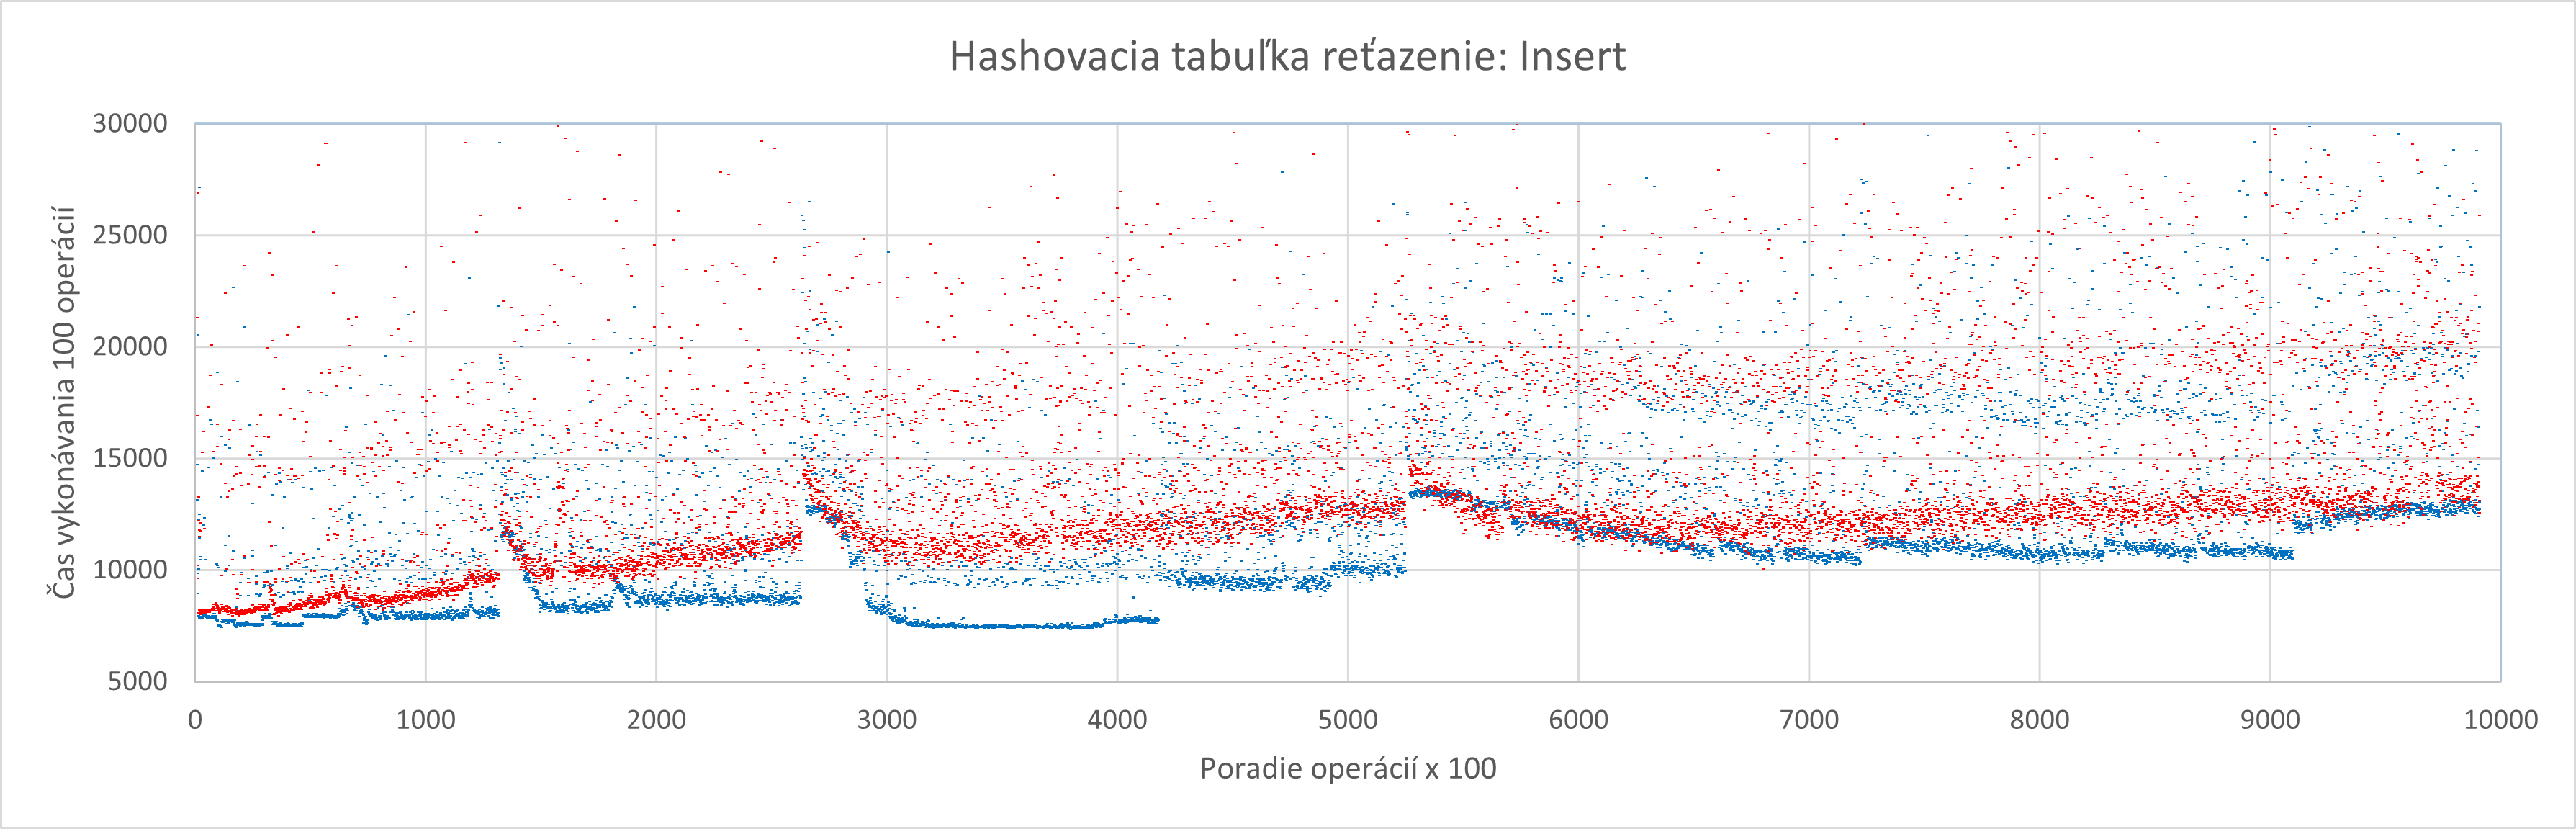
\includegraphics[width=\textwidth]{HashSC_Insert_zoomed}
    \end{figure}

    \FloatBarrier

    \newpage
    \FloatBarrier

    \includepdf[pages=-,offset= 0 -2cm, scale = .98,pagecommand=\section{Príloha A - Zadanie č.2 Vyhľadávanie v dynamických množinách}\label{sec:priloha-a-zadanie-c-2-vyhladavanie-v-dynamickych-mnozinach}]{DSA_zadanie2.pdf}

    \newpage


    \section{Príloha B – Upresnenie znenia zadania č. 2}\label{sec:priloha-b-upresnenie-znenia-zadania-c-2}
    \begin{itemize}
        \item {\makebox[8.5cm]{vlastná implementácia BVS\hfill}  – 02 body
            \begin{itemize}
                \item vyvažovanie
            \end{itemize}
            \item {\makebox[8.5cm]{vlastná implementácia hash tabuľky\hfill} – 02 body
                \begin{itemize}
                    \item riešenie kolízií
                    \item zväčšovanie tabuľky
                \end{itemize}
                \item {\makebox[8.5cm]{prevzatá implementácia BVS\hfill} – 01 bod
                \item {\makebox[8.5cm]{prevzatá implementácia hash tabuľky\hfill} – 01 bod
                \item  {\makebox[8.5cm]{testovací program\hfill} – 02 body
                    \begin{itemize}
                        \item vytvoriť BVS/hash o veľkosti počtu prvkov 1 000/25 000/100 000
                        \item používajte rovnaké prvky pre BVS aj has tabuľku
                        \item operácia insert - čas potrebný na:
                        \begin{itemize}
                            \item vytvorenie
                            \item 1 prvok
                            \item 25 \% prvkov
                            \item zopakujte 5 krát
                        \end{itemize}
                        \item operácia search - čas potrebný na:
                        \begin{itemize}
                            \item 1 prvok
                            \item 5 \% prvkov
                            \item zopakujte 5 krát
                        \end{itemize}
                    \end{itemize}
                    \item {\makebox[8.5cm]{dokumentácia\hfill}                    – 02 body
                        \begin{itemize}
                            \item opisy algoritmov
                            \item spôsob testovania
                            \item dosiahnuté výsledky
                        \end{itemize}
                        \item {\makebox[8.5cm]{celkom:\hfill}    – 10 bodov
    \end{itemize}


\end{document}